\documentclass[a4paper,10pt]{scrartcl}
\usepackage{mathe-vorlesung}
\usepackage{graphicx}
\renewcommand{\equiv}{\Longleftrightarrow}
\newcommand{\eps}{\varepsilon}
\newcommand{\del}{\delta}
\newcommand{\homo}{\stackrel = \sim}

\title{Topologie}

\begin{document}

\maketitle

\tableofcontents
\newpage
\begin{center}
\LARGE\textbf{Vorwort}
\end{center}
\begin{seg}{Was ist Topologie?}
\begin{itemize}
\item "` Unterzeichnung geometrischer Objekte bis auf stetige Dekorationen. "'
\item "` Stetigkeitsgeometrie"', "` qualitative Geometrie "', "`Gummi-Geometrie"'
\end{itemize}
Objekte werden in der Topologie als gleich angesehen, wenn sie durch eine in beiden Richtungen stetige bijektive Abbildung aufeinander abgebildet werden kann ("` Homöomorphismus"').
\end{seg}
So zum Beispiel für Teilmengen des $\R^2$:
\begin{figure}[h]
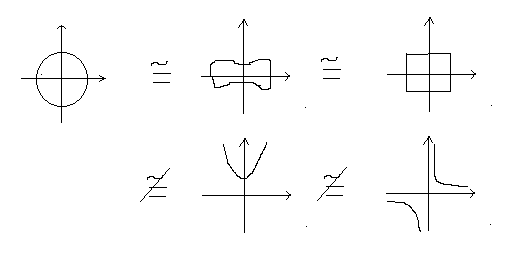
\includegraphics[scale=0.7]{fig1.png}
\end{figure}
\begin{ex*} 
Topologische Begriffe sind beispielsweise \emph{Stetigkeit, offene/abgeschlossene Mengen, Umgebung, Rand, Abschluss, Konvergenz, kompakt, zusammenhängend, Homotopie}.  Die konkreten Definition werden im Verlauf dieser Vorlesung geklärt.
\end{ex*}
\begin{center}
\LARGE\textbf{I Grundbegriffe}
\end{center}
\section{Metrische und topologische Räume}
\begin{df}
Ein \emph{metrischer Raum} ist eine Menge $X$k zusammen mit einer Funktion $d: X \times X \rightarrow \R$, genannt Metrik oder \emph{Abstandsfunktion}, so dass folgende Axiome gelten:
\begin{enumerate}[\roman{enumi})]
\item \emph{Positivität}: $d(x,y)\ge 0 \land d(x,y)=0\equiv x=y$
\item \emph{Symmetrie}: $d(x,y)=d(y,x)$
\item \emph{Dreiecksungleichung}: $d(x,z) \le d(x,y)+d(y,z)$
\end{enumerate}
\end{df}
\begin{ex*}
Auf $\R^n$ ist durch die \emph{Euklidische Norm} $|x|=\sqrt{x_1^2+...+x_n^2}$ die \emph{Euklidische Abstandsfunktion} $d(x,y)=||x-y||$ gegeben. Auf $\R$ oder auf $\C$ ist diese Metrik durch den Betrag $d(x,y):=|x-y|$ definiert.  Man erhält auf diese Weise aus jeder Norm eine Metrik. Hierbei liefern verschiedene Normen natürlich verschiedene Metriken. Hier einige Beispiele auf $\R^2$:
\begin{itemize} 
\item euklidische Norm: $||x||_2=\sqrt{x_1^2+x_2^2}$
\item Maximumsnorm: $||x||_\infty := \max(|x_1|, |x_2|)$
\item $\Eins$-Norm $||x||_1 := |x_1|+|x_2|$
\end{itemize}
\end{ex*}

\begin{ex*}
Die diskrete Metrik definiert durch:
\[
d(x,y)=\begin{cases}
  0, & \text{falls} x=y \\ 1, & \text{falls} x\neq y
\end{cases}
\]
\end{ex*}

Es lassen sich zwei zentrale mathematische Begriffe mit HIlfe von Abstandsfunktionen definieren:
\begin{itemize}
\item Konvergenz von Folgen
\item Stetigkeit von Abbildungen
\end{itemize}

\begin{df}[Konvergenz im metrischen Räumen]
Sei $X$ ein metrischer Raum und $x_N, n\in \N$ eine Folge in $X$. Wir sagen $(x_n)_{n\in \N}$ \emph{konvergiert}, falls es ein $a \in X$ gibt, so dass gilt:
\[
\forall_{\varepsilon>0}\exists_{k\in\N}\forall_{n\ge k}: d(x_n,a)<\varepsilon
\]
\end{df}
In diesem Fall sagen wir, $a$ ist der \emph{Limes} (oder Grenzwert) von $(x_n)_{n\in \N}$ (und schreiben $x_n\rightarrow a, \lim\limits_{n\rightarrow \infty} x_n=a$) 

\begin{st} In einem metrischen Raum ist der Limes eine konvergente Folge eindeutig bestimmt.
\end{st}
\begin{proof}
Seien $a$ und $b$ Limiten von $(x_n)_{n\in \N}$ mit $\delta := d(a,b)>0$.

Da $(x_n)_{n\in \N}$ gegen $a$ konvergiert, gibt es $k\in \N$, sodass $d(x_n,a)<\frac{\delta}{2}$ für alle $n \ge k$.
Dann gilt nach Dreiecksungleichung:
\[
\delta=d(a,b)\le \underbrace{d(x,x_n)}_{<\frac{delta}{2}}+d(x_n,b)
\]
Also gilt $d(x_n,b)\ge \frac{\delta}{2}$ für alle $n\ge b$, was der Konvergenz gegen $b$ widerspricht.
\end{proof}
\begin{df}[$\eps$-$\delta$-Definition der Stetigkeit in metrischen Räumen]
Seien $X$ und $\tilde X$ metrische Räume mit Abstandsfunktion $d$ bzw. $\tilde d$. Eine Abbildung $f: X \rightarrow \tilde X$ heißt stetig in$x \in X$ falls gilt: 
\[\forall_{\eps>0}\exists_{\delta>0} \forall_{x'\in X}: d(x,x')<\delta \implies \tilde d(f(x), f(x'))<\eps\]

Die Abbildung heißt \emph{stetig}, falls dies für alle $x\in X$ gilt.  Stetigkeit in metrischen Räumen hängen eng zusammen. Es gilt:
\end{df}
\begin{st}
Eine Abbildung $f: X\rightarrow \tilde X$ zwischen metrischen Räume ist genau dann stetig, wenn für jede konvergente Folge $x_n \rightarrow a$ in X gilt, dass $f(x_n) \rightarrow f(a)$
\end{st} 
\begin{proof}
\begin{seg}{"`$\implies$"'}
Sei $\eps>0$, dann gibt es $\delta>0$, so dass aus $d(x',a)<\delta$ folgt: $d(f(x'),f(a))<\eps$. Weiter gibt es ein $k\in \N$, so dass $d(x_N,a)y\delta$ für $n \ge k$.  Insgesamt folgt $d(f(x_n),f(a))<\eps$ für alle $n\ge k$.
\end{seg}
\begin{seg}{"`$\Longleftarrow$"'}
Angenommen, $f$ ist nicht stetig. Dann gibt es ein $x \in X$ und ein $\eps>0$, so dass es zu jeden $n\in \N$ ein $x$ mit $d(x_n,x)<\frac{1}{n}$ und $d(f(x_1), f(x))\ge \eps$ gibt. Damit ergibt sich der Widerspruch.
\end{seg}
\end{proof}
Die obigen Definition lassen sich mit Hilfe von $\eps$-Bällen umformulieren:
\begin{df}
Sei $X$ ein metrischer Raum und $x\in X$, dann heißt die Teilmenge 
\[
B_\eps(x)={x'\in X|d(x',x)<\eps}
\]
von $X$ heißt der (\emph{offene}) \emph{Ball mit Radius $\eps$ um x} (kurz: \emph{$\eps$-Ball}).
\end{df}
\begin{df}
In einem metrischen Raum heißt eine Teilmenge $U\subset X$ \emph{offen}, wenn es um jeden ihrer Punkte einen offenen $\eps$-Ball gibt, der ganz in U enthalten. Eine Teilmenge A heißt \emph{abgeschlossen}, wenn ihr Komplement $X\setminus A$ offen ist.  Eine Teilmenge $U \subset Y$ heißt \emph{Umgebung} eines Punktes $ x\in X$, falls es eine offene Teilmenge $V \subset X$ gibt mit $x\in v$ und $V \subset U$.  (Äquivalent: falls es ein $\eps$ mit $B_\eps(x)\subset U$ gibt.  
\end{df}

\begin{figure}[h]
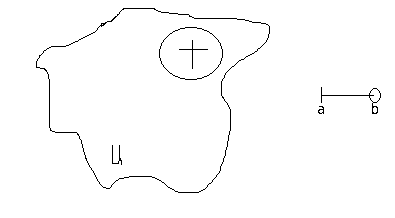
\includegraphics[scale=0.5]{fig3.png}
\end{figure}

Konvergenz und Stetigkeit lassen sich in metrischen Räumen durch offene Mengen beschreiben.
\begin{st}
In einem metrischen raum konvvergiert eine Folge $(x_n)_{n \in \N}$ genau dann gegen x, wenn es zu jeder Umgebung $U$ von $x$ ein $k \in \N$ gibt, so dass $x_n \in U$ für alle $n \ge k $ gilt.\\
\underline{Kurz:} Eine Folge $(x_n)_{n \in \N}$ konvergiert gegen $x$, wenn in jeder Umgebunng von $x$ \emph{fast alle} ($\hat =$ alle bis auf endlich viele) Folgenglieder liegen.
\end{st}
\begin{proof}
Die Äwuivalenz gilt, da jede Umgebung von $x$ einen $\eps$-Ball um $x$ enthält und umgekehrt jeden $\eps$-Ball um $x$ auch eine Umgebung von $x$ ist.
\end{proof}
\begin{st}\label{st:1.8}
Eine Abbildung zwischen metrischen Räumen $f: X\rightarrow \tilde X$ ist genau dann stetig in $x \in X$, wenn es zu jeder Umgebung $V$ von $f(X)$ eine Umgebung $U$ von $x$ gibt, so dass U unter $ f $ in V abgebildet wird; oder äquivalent dazu, falls das Urbild jeder Umgebung von $  f(x) $ eine Umgebung von x ist.
\end{st}
\begin{proof}
Dies folgt direkt aus der $ \eps $-$ \delta $-Definition der Stetigkeit und er Definition der Umgebung.
\begin{figure}[h]

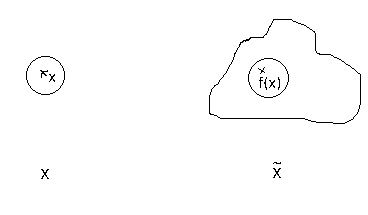
\includegraphics[scale=0.5]{fig4.png}
\end{figure}
\end{proof}
\begin{st}
Eine Abbildung zwischen metrischen Räumen ist stetig genau dann, wenn die Urbilder offener Mengen offen sind.
\end{st}
\begin{proof}
\begin{seg}{"`$\Longrightarrow$"'}
Sei $ f: X \to \tilde X $ stetig und $ V \subset \tilde Y $ offen.  Dann ist $ f^{-1}(V) $ nach \ref{st:1.8} eine Umgebung jeder ihrer Punkte somit offen.
\end{seg}
\begin{seg}{"`$\Longleftarrow$"'}
Seien umgekehrt die Urbilder offener Mengen offen und $ x \in X $. Sei $ \eps>0 $.  Nach Voraussetuuimg $ f^{-1}(B_\eps(f(x)) $ offen und enthält somit einen $ \delta $-Ball um den Punkt x.
\end{seg}
\end{proof}

Wichtige Beobachtung: Um KOnvergenz und Stetigkeit zu beschreiben muss man nicht direkt auf eine Metrik Bezug nehmen, sondern es genügt das System der offenen Mengen zu kennen.  Dieses System von offenen Mengen nennt man \emph{die Topologie} des metrischen Raums .  Verschiedene Metriken können dieselbe Topologie erzeugen.

Alle Eigenschaften von metrischen Räumen, ihren Teilmengen oder Abbildung zwischen metrischen Räumen, die sich durch die Topologie (ohne direkten Bezug auf die metrik) beschreiben lassen, nennen wir \emph{topologische Eigenschaften}.

Dies führt zu dem folgenden Begriff:
\begin{df}
Sei $ X $ eine Menge und $O \in \mathcal P (x)$ eine Menge von Teilmengen von X; $ O $ heißt eine \emph{Topologie} auf $ X $, wenn folgendes gilt:
\begin{itemize}
\item[(T1)] Beliebige Vereinigungen von Mengen in $ O $ liegen wieder in O.
\item[(T2)] Die Schnittmenge von je zwei Mengen in $  O  $ liegt
\item[(T3)] Es gilt $ \emptyset \in O $ und $ X \in O$
\end{itemize}
Eine Menge $ X $ zusammen mit einer Topologie auf $ X $ heißt \emph{topologischer Raum}, die Elemente von $ O $ nennt man \emph{offene Teilmengen} von X, ihre Komplemente \emph{abgeschlossene Teilmengen}.
\end{df}
\begin{note*}
\begin{enumerate}[(\roman{enumi})]
\item Natürlich ist die Definition so gemacht, dass die in einem Topologie bilden.
\item Verschiedene Metriken können diesselbe Topologie erzeugen, vgl. der aus der Analysis bekannter Satz, dass alle Normen auf dem $ \R^n $ äquivalent.  Daraus folgt: die Metrik die Metrik $ d(x,y) :=||x-y|| $ definiert für \emph{alle Normmen auf $ \R^n $} dieselbe Topologie, die sogenannte \emph{Standardtopologie}, zum Beispiel definieren:
\begin{align*}
d_1(x,y)&=|x_1-y_1|+...+|x_n-y_n|\\
d_2(x,y)&=\sqrt{(x_1-y_1)^2+...+(x_n-y_n)^2}\\
d_\infty(x,y)=\max(|x_1-y_1|, ..., |x_n-y_n|)
\end{align*}
alle die Standardtopologie.
\end{enumerate}
\end{note*}
\begin{df}
Sei $ X $ ein topologischer Raum und  $x \in X $ Eine Teilmenge $ U \subset X $ heißt \emph{Umgebung} von x, wenn es eine offene Menge $ T\subset U $ gibt, die $ x $ enthält.  $ x $ heißt \emph{innerer Punkt} von A, wenn $ A $ eine Umgebung von $ x $ ist. $ x $ heißt \emph{äußerer Punkt}, falls $ X\setminus A $ eine Umgebung von x ist. Der Punkt $ x $ heißt Randpunkt von $ A $, falls keine von beiden gilt.  Die Menge $ \mathring{A} $ der inneren Punkte von $ A $ bezeichnet man als das \emph{Innere} von $ A $ oder als \emph{offener Kern} von $ A $. Die Menge $ \bar A $, der nichtäußeren Punkte von $ A $ heißt \emph{Abschluss} oder \emph{abgeschlossene Hülle} von $ A $.  Die Menge der Randpunkte von $  A $  heißt auch der Rand von A und wird mit $ \delta A $ bezeichnet. 
\end{df}

\begin{ex*}
Sei $ A=[a,b)\subset \R $ und sei $\R$ mit der Standardtopologie versuchen.  Dann gilt $\mathring A=(a,b), \bar A=[a,b], \delta A={a,b}, B=\Q\subset \R$ gilt $ \mathring B=\emptyset, \bar B=\R, \delta B=\R $ 
\end{ex*}
\begin{ex}[Beispiele für Topologien]\label{thm:1.12}
\begin{enumerate}[(\roman{enumi})]
\item Durch Metriken definierte Topologie. Dies sind die sogenannten \emph{metrisierbaren Topologien}.
\item Die \emph{Klumpentopologie} $ O=\{\emptyset, X\} $ für eine beliebige Menge $ X $.  Sie ist nicht metrisierbar (falls $ X $ mehr als ein Element hat)
\item Die \emph{diskrete Topologie} $ O=\mathcal{P}(x) $ ist für jede beliebige Menge $ X $ definiert.  (Nur die schließlich konstanten Folgen sind konvergent.) Sie ist durch die diskrete Metrik gegeben.
\item Auf $\R^2$ ist durch
\[
O=\{A\subset \R^2|\forall_{(x,y)\subset A}\exists_{\eps>0}:(x-\eps,x+\eps) \times \{y\} \subset A\}
\]
eine Topologie gegeben. Übung: Ist diese metrisierbar?
\end{enumerate}

\end{ex}

\begin{df}
Sind auf einer Menge $X$ zwei Topologien $ O_1$ und $ O_2 $ gegeben, dann betrachten wir folgende Sprachweisen: gilt $ O_1 \subset O_2 $ , dann sagen wir $ O_2 $ ist \emph{feiner} als $ O_1 $ (und $ O_1 $ ist \emph{gröber} als $ O_2 $).  Gilt weder $ O_1 \subset O_2 $ noch $ O_2\subset O_1 $ , dann sagen wird, die Topologien $ O_1 $ und $ O_2 $ sind \emph{unvergleichbar}.
\end{df}

Auf jeder Menge ist die Klumpentopologie die größte mögliche Topologie und die diskrete Topologie, die feinst mögliche Topologie.  Die Topologie in \ref{thm:1.12}(iv) auf $ \R^2 $ ist feiner als die Standardtoplogie, aber gröber als die diskrete.

\begin{df}
Sei $ X $ ein topologischer Raum.  Eine Folge $ x_n $ heißt konvergent gegen $ a\in X $, falls jede Umgebung von $ a $ fast alle Folgenglieder enthält.
\end{df}
\begin{df}
Eine Abbildung $ f:X\to Y $ zwischen topologischen Räumen heißt \emph{stetig} in $ x\in X $, falls es zu jeder Umgebung $ V $ von $ f(x) $ eine Umgebung $ U $ von $ x $ gibt, so dass $ f(U)\subset V $ (Äquivalent: Falls das Urbild jeder Umgebung von $ x $ ist.) Die Abbildung heißt \emph{stetig}, wenn die Urbilder offener Mengen offen sind. Eine Abbildung zwischen topologischen Räumen, die bijektiv und stetig ist, heißt \emph{Homöomorphismus} (falls auch ihre Umkehrabbildung stetig ist.  Falls es einen Homöomorphismus $ d: X\to Y $ gibt, sagt man, $ X $ und $ Y $ sind \emph{homöomorph}, man schreibt: $ X\homo Y $.
Aus der Definition folgt sofort, dass eine Abbildung. $ f: X\to Y $ genau dann stetig ist, falls sie in jedem $ x\in X $ stetig ist. (zur Übung nachvollziehen)
\end{df}
\begin{st}
Sei $ f: X\to Y $ eine (in $ a\in X $) stetige Abbildung zwischen topologischen Räumen.  Sei $ x_n\to a $ konvergente Folge in $ X $. Dann gilt $ f(x_n) \to f(a) $
\end{st}
\begin{proof}
Sei $ V $ eine Umgebung von $ f(a) $. Da $ f $ (in $ a $) stetig ist, ist $ f^{-1}(V) $ eine Umgebung von $a$.  Wegen $ x_n\to a $ liegen fast alle $ x_n $ in $f^{-1}(V)$, somit gilt für fast alle $f(x_n)$ in $ V $.
\end{proof}
\begin{att}
Eine Abbildung, die jede konvergente Folge auf eine gegen das Bild des Limes konvergierende Folge abbildet (so eine Abbildung heißt \emph{folgenstetig}) ist \emph{im Allgemeinen nicht} notwendigerweise stetig. Siehe z. B. Joerich "`Topologie"' 6.3, bzw. später in der Vorlesung.
\end{att}
\begin{ex*}
\begin{enumerate}[(i)]
\item ist $ f: X\to Y $ eine stetige Abbildung und wird die Topologie auf X durch eine feinere oder die Topologie auf X durch eine gröbere ersetzt, bleibt $ f $ stetig.
\item Insbesondere ist \emph{jede} Abbildung $ f: X\to Y $ stetig falls $ Y $ die Klumpentopologie oder $ X $ die diskrete Topologie trägt.
\item In der Klumpentopologie ist \emph{jede} Folge gegen \emph{jeden Punkt} konvergent. 
\end{enumerate}
\end{ex*}
\begin{note}
Die Axiome eines topologischen Raums sind für sich alleine relativ schwach und lassen sich und lassen sehr viele Beispiele auch mit "pathologischen" Eigenschaften zu. Sie sind eher ein äußerer Begriffsrahmen. Um etwa Räume mit den von metrischen Räumen vertrauten Eigenschaften zu erhalten, muss man Zusatzannahmen machen.
\begin{itemize}
  \item "`Hausdorffeigenschaft"' $\implies$ Eindeutigkeit des Limes
  \item "`Abzählbarkeitsaxiome"' $\implies$ Äquivalenz von Stetigkeit und Folgendefinition
\end{itemize}
\end{note}
\section{Grundkonstruktionen}
Grundkonstruktionen sind Methoden, um neue Topologien zu definieren durch:
\begin{itemize}
\item Summe, teilräume, Produkte, Quotienten
\item durch Abbildungen zwischen topologischen Räumen
\end{itemize}
\begin{df}
Seien $ X $ und $ Y $ topologische Räume. Auf der disjunkten Vereinigung $ X \dot \cup V =X \times \{ 0 \} \cup Y \times \{1\}$ definieren wir eine Topologie durch:
\[
\{U \mathbin{\dot{\cup}} V| U \text{ offen in } X, V \text{ offen in } Y\}
\]
Der so entstehende topologische Raum $ X+Y $ wird als topologische Summe von X und Y bezeichnet (andere übliche Zeichen: $X \sqcup Y$ oder auch $X \perp Y$).
\end{df}
\begin{note*}
\begin{enumerate}[(i)]
\item Analog definert man die Summen von beliebig (auch unendlich) vieler topologischer Räumen $\biguplus_{\alpha \in  A} x_\alpha=\bigsqcup_{\alpha\in A} x_\alpha$, widerum als offene Menge $\{\dot \bigcup_{\alpha\in A}| U_\alpha \text{ offen in } X_\alpha \}$ setzt.
\item Für die disjunkte Verreinigung von Mengen $ X \dotcup Y $ ist auch die Schreibweise $X+Y:= X\times\{0\} \cup Y\times \{1\}$ üblich.  
\end{enumerate}
\end{note*}
\begin{ex*}
\begin{enumerate}[i]
\item Sei $ X=\{ x\} $ eine einelementige Menge. Dann ist die topologische Summe $ \biguplus_{\alpha\in A}X_\alpha $
\item Beispiel \ref{thm:1.12}(iv) ist homöomorph zu $ \biguplus_{\alpha\in \R} X_\alpha \R $ (Übung)
\end{enumerate}
\end{ex*}
\begin{df} Sei $ X $ ein topologischer Raum und $ M \subset X $. Die durch $ \{ U\cap M| U \text{ offen in } X \}$ auf $M$ defnierte Topologie heißt $ Teilraumtopologie $ (auch \emph{induzierte}, \emph{Relativ-} oder \emph{Spurtopologie}). 
\end{df}
\begin{ex*}
$X=\R^2, M=\{x-\text{Achse}\}$
\fixme{figure}
\end{ex*}
\begin{att*}
Die offene Mengen $U\cap M$ in $ M $ sind im Allgemeinen nicht offen in $ X $ (es sei denn $ M\subset X $ wäre offen). Zum Beispiel:
\[
\text{T2: } (\underbrace{U_1}_{\text{offen in }X}\cap M)\cap (\underbrace{U_2}_{\text{offen in }X}\cap M)=(U_1\cap U_2)\cap M
\]
\end{att*}
\begin{df}
Seien $ X $ und $ Y $ topologische Räume. Eine Teilmenge $ W\subset X\times Y $ heißt offen bezüglich der Produktopologie auf $ X\times Y $ heißt offen bezüglich der Proudukttopologie auf $X\times Y$, falls es zu jedem Punkt $ (x,y)\in W $ eine Umgebung $ U $ von $ x $ und eine Umgebung $ V $ von $ y $ gibt, sodass $ U\times V $ in W enthalten ist.
\fixme{figure}
\end{df}
\begin{note*}
\begin{enumerate}[(i)]
\item Die Standardtopologie auf $ \R^2 $ stimmt mit der Produkttopologie auf $ \R\times \R $ (beide Faktoren mit der Standardtopologie von $ \R $ versehen) überein.
\item Produkte offener Mengen in X und Y ("`Kästchen"') sind offen in den Produkttopoligien, aber nicht alle offenen Mengen sind Kästchen, z. B. sind auch die Vereinigung von Kästchen Kästchen.
\fixme{figure} 
\end{enumerate}
\underline{Erinnerung:} Eine \emph{Äquivalenzrelation} auf einer Menge $ X $ ist eine Relation $\sim$ mit folgenden Eigenschaften:
\begin{enumerate}[(i)]
\item reflexiv: $a\sim a$
\item symmetrisch: $a\sim b \implies b\sim a$
\item transitiv: $a\sim b \land b \sim c\implies a\sim c$
\end{enumerate}
ist auf einer Menge $ X $ eine Äquivalenzrelation $\sim$ gegeben, so liegt jedes Element in seiner Äquivalenklasse
\[
 [x]:=\{y\in X|x\sim y\} \subset X
\]
und Äquivalenzklassen von zwei verschiedenen Elemente sind entweder disjunkt oder gleich; M zerfällt in die disjunkte Vereinigung der Äquivalenzklassen.  umgekehrt liefert eine Zerlegung einer Menge in disjunkte Teilmengen eine Äquivalenzrelation.
\end{note*}
\begin{df}
Sei X ein topologischer Raum und $\sim$ eine Äquivalenzrelation auf $ X $.  Sei $X/\sim$ die Menge der Äquivalenzklassen 
\[
X/\sim=\{[x]|x\in X\}
\]
und sei $ q: X\to X/\sim, x\mapsto [x] $ eine Teilmenge $ U $ von $ X/\sim $ ist genau dann offen bezüglich der \emph{Quotiententopologie} auf $ X/\sim $, wenn ihr Urbild $ q^{-1}(U) $ offen in X ist.
\end{df}

\begin{ex*}
\begin{enumerate}[(i)]
\item \begin{seg}{Zusammenschlagen eines Teilraums zu einem Punkt}
Sei $ X $ ein topologischer Raum und $ A\subset X $ ein Teilraum. Dann ist durch $ x \sim y :\equiv (x=y)\lor (x,y\in A) $ eine Äquivalenzrelation gegeben.  Zwei Punkte werden als äquivalent angesehen, wenn sie gleich sind oder beide in $ A $ liegen.
\end{seg}
\item \begin{seg}{Beispiel zu (i)}
Sei X ein topologischer Raum. Betrachte $ X\times [0,1] $
\fixme figure
Man erhält den Kegel $CX:=X\times[0,1]/X\times\{1\}$
\end{seg}
\item Allgemeiner: "`\emph{Zusammenkleben}"'
\begin{enumerate}[(a)]
\item \fixme figure
\item \fixme figure
\end{enumerate}
bei (b) handelt es sich nicht um Zusammenschlagen eines Teilraums zu einem Punkt, sondern gegenüberliegend Punkte in den beiden senkrecht "`Radintervalle"' werden identifiziert mit den Äquivalenzrelationen:
\[
(x_1,x_2)\sim (y_1,y_2):\equiv (x_1,x_2)=(y_1,y_2)\lor (x_1,y_1 \in \{0,1\} \land x_2 =y_2)
\]
\end{enumerate}
\end{ex*}
Eine weitere Möglichkeit aus gegebenen topologischen Räumen andere zu konstruieren, ist es, Topologien mit Hilfe von Abbildungen zu übertragen.
\begin{df}\label{thm:2.5}
\begin{enumerate}[(i)]
\item Sei $ X $ ein topologischer Raum und $ X $ eine Menge.  Sei $ f: X\to Y$ eine Abbildung.  Dann ist durch:
\[
\{U\subset Y|f^{-1}(U) \text{ offen} \}
\]
die \emph{finale Topologie} auf Y definiert.
\item Sei $ X $ eine Menge und $ X $ ein topologischer Raum.  Sei $ f: X\to Y $ eine Abbildung.  Dann ist durch 
\[
\{ f^{-1}(U)\subset X| U \text{ offen in } Y\}
\]
die \emph{initiale Topologie} auf X definiert.
\end{enumerate}
\end{df}
\begin{note*}
Die \emph{finale Topologie} ist die feinste Topologie auf Y die f stetig macht in (i). In (ii) ist die initiale Topologie die gröbste Topologie auf $ X $, die f stetig macht.
\end{note*}
\begin{exs*}
\begin{enumerate}[(i)]
\item Die Teilraumtopologie auf $M\subset X$ ist die initale Topologie bezüglich der \emph{Inklusionsabbildung} $ i:M\to X,m\mapsto m $, denn es gilt $ i^{-1}(U)=U\cap M $ für (offene) Mengen in $ X $.
\item Die Quotientenabbildung ist die finale Topologie bezüglich der Quotientenabbildung ist die finale Topologie bezüglich der Quotientenabbildung $ q: X\to X/\sim, x\mapsto [x] $
\item in ähnlicher Weise lässt sich die Summentopologie charakterisieren.  Sie ist die feinste Topologie, so dass beide Inklusionsabbildungen
$ i_X:X\to X+Y, x \mapsto x, i_Y: Y\to X+Y,y\mapsto y $ stetig sind.  Dies zeigt, dass es sinnvoll ist die Defnition \ref{thm:2.5} noch etwas weiter zu fassen.
\end{enumerate}
\end{exs*}
\begin{seg}{Zusatz zu Definition \ref{thm:2.5}}\label{thm:2.5(2)}
Allgemeiner definieren wir:
\begin{enumerate}[(i)]
\setcounter{enumi}{2}
\item Seien $X_i, i\in I$ topologische Räume und $ Y $ eine Menge. Sei durch $f_i:X_i\to Y, i\in I$ eine Familie von Abbildungen gegeben. Die feinste Topologie auf $ Y $, die alle Abbildungen $f_i$ stetig macht, heißt finale Topologie bezüglich $ f_i,i\in I $.
\[
\{U\subset Y|f^{-1}_i(U) \text{ offen in }X_i \text{ \emph{für alle}} i\in I\}
\]
$(T1) U_1, U_2\in O$ zeige: $U_1\cup U_2\in O$
\[f^{-1}(U_1\cup U_2)=\underbrace{f^{-1}_i(U_1)}_{\text{offen in } X_i}\cup \underbrace{f^{-1}_i(U_2)}_{\text{offen in } X_i}\]
\item Seien $ Y_i, i\in I $, topologische Räume und $ X $ eine Menge.  Seien $ f_i: X\to Y_i $ Abbildungen.  Die gröbste Topologie auf $ X $, die alle $f_i$ stetig macht, nämlich $\{f^{-1}_i\subset X| U \text{ offen in } Y, i\in I\}$ ist die \emph{initiale Topologie} bezüglich $f_i$. 
\end{enumerate}
\end{seg}
\begin{ex*}
Die Produkttopologie auf $ X\times Y $ ist initiale Topologie bezüglich der bei den kanonischen Projektionen
\[
\pi_X:X\times Y \to X, (x,y)\to x \text{ und } \pi_Y: X\times Y\to Y, (x,y)\to y 
\]
\end{ex*}
\end{document}
